\section{Week 2 : Client Server}

\subsection{Server Client}
Distributed computing involves multiple independent computational entities (nodes) that communicate over a network to achieve a common goal.  A fundamental model is the client/server architecture, where:
\begin{enumerate}[noitemsep]
    \item Client: Initiates requests for services.
    \item Server: Processes requests and provides responses.
\end{enumerate}

This is a fundamental concept used every day. For example, ordering food means that you are a client talking to a server. Other examples are web or mail servers.

\subsection{Design Issues}
These issues are primarily addressed later in the course, but an introduction is provided here.

\subsubsection{Division of Labour}
\textbf{Concept:} How to divide the overall task into smaller, manageable subtasks that can be executed concurrently by different nodes.

\textbf{Theoretical Foundation:}  \href{https://en.wikipedia.org/wiki/Amdahl\%27s_law}{Amdahl's Law} provides a theoretical limit on the speedup achievable through parallelization. It highlights the importance of minimizing the sequential portion of a task.

\textbf{Practical Implication:} Careful task decomposition is crucial for scalability.  Overly fine-grained tasks can lead to excessive communication overhead, while overly coarse-grained tasks may not fully utilize available resources.

\textbf{Industry Application:}  MapReduce (used by Google) is a prime example.  A large dataset is split into smaller chunks (\texttt{"map"} phase), processed independently, and then the results are combined (\texttt{"reduce"} phase).


\subsubsection{Reliability of Transmission}
\textbf{Concept:} Ensuring data transmitted between nodes arrives correctly and in the intended order, despite potential network failures.

\textbf{Theoretical Foundation:}  \href{https://en.wikipedia.org/wiki/Two_Generals\%27_Problem}{The Two Generals' Problem} demonstrates the fundamental impossibility of achieving perfect agreement in the presence of unreliable communication channels.

\textbf{Practical Implication:} Reliable communication protocols (e.g., TCP) use techniques like acknowledgments, retransmissions, and checksums to detect and correct errors.  However, these add overhead. In the example presented in the class, if a network is working all the time, if the server is online and functioning properly, and if the messages are not getting lost, the transmission is reliable.

\textbf{Industry Application:} \textit{TCP/IP}, the foundation of the internet, provides reliable, ordered byte streams.  Higher-level protocols (e.g., HTTPS) build on this foundation.


\subsection{Server Design}

Server design often involves transparency.  This means that multiple machines can respond to a user's request, but they share a common endpoint. The user interacts with this single point, unaware of the underlying complexity. This is achieved using a load balancer, which acts as a traffic director. The load balancer is a device or software that distributes network or application traffic across multiple servers.  This distribution prevents any single server from becoming overwhelmed, improving the responsiveness and availability of applications, and ensuring reliability and high performance.

%\begin{figure}[h]
%    \centering
%    \includegraphics[width=0.5\textwidth]{./imgs/server_design_week2.jpeg}
%    \caption{Figure: Server Design Transparency}
%\end{figure}

\subsection{Managing State}

State Management is crucial between the client and the server. For example, in an email client, emails are stored on the server and should be accessible from anywhere at any time. If a user goes offline, the server and the client need to determine which emails the user has and hasn't accessed.  Furthermore, in server-server communication, data across all servers must be synchronized and up-to-date.

\begin{enumerate}[itemsep=1pt]
    \item \textbf{Stateful Server:} The server maintains the state.  Clients are typically thin.  This simplifies client logic but can create a single point of failure and a bottleneck.
    \item \textbf{Stateless Server:} The server does not store any client-specific state between requests. Each request must include all necessary information. This improves scalability and fault tolerance but increases message size and complexity.
    \item \textbf{Shared State:}  A hybrid approach where some state is managed by the server, and some may be managed by the client or a separate distributed data store.
\end{enumerate}

\subsection{Concurrency}
Concurrency refers to events happening simultaneously, often in an unpredictable order. When order is important, operating system concepts like locks are used to manage concurrent access to shared resources. Locks ensure that only one process can access a resource at a time, preventing data corruption and inconsistencies.

\subsection{Work Distribution}
Work distribution involves balancing the load across servers. This includes considering the number of clients each server handles, their memory load, processor load, and overall client interaction.

\subsection{State}
A state represents a piece of information. For example, if two web servers handle client requests and a user is logged in, this status (e.g., \texttt{UserLoggedIn=true}) must be maintained on both machines. A state machine transitions through different states.  For instance, a user login might involve inputting a password, then proceeding to 2-factor authentication (2FA), and finally achieving a logged-in state.  A stateful machine stores state information in the server-client connection or even in server-server interactions.  For instance, a learning management system (LMS) server might store user IDs, interaction history, duration of interactions, IP addresses, and browser information. On the client side, a cookie can store state information, such as language preferences.  A stateless machine, on the other hand, does not store any state. Examples include simple HTTP servers and DNS servers.  TCP maintains a connection state, storing information about connected hosts. UDP, used for live streaming and video calls, does not maintain connection state; the order of packets is not guaranteed.

\subsubsection{Case Study: Network File System (NFS)}

If two different machines can write to files on the same server, file locking is necessary.  The server maintains state information about which machine has a lock on a file.  In the example below, the server holds the state indicating which machine first requested to edit the file. Only changes from that machine are executed; other requests fail. The NFS server is a stateful machine, holding the locks on files.  However, if the NFS server fails before completing a write operation, the lock might persist, leading to inconsistencies. This illustrates a trade-off between stateful and stateless designs. In practice, NFS servers employ complex solutions to manage state and handle potential failures.

%\begin{figure}[h]
%    \centering
%    \includegraphics[width=0.4\textwidth]{./imgs/NFS_serverl2.jpeg}
%    \caption{Figure: Example of NFS server using states}
%\end{figure}

\subsubsection{Case Study: UM Learn}

UM Learn (a learning management system) exhibits state transitions. A user might transition from a "not logged in" state to a "2FA" state and finally to a "logged in" state.  A failed 2FA attempt might return the user to the "not logged in" state.

\subsubsection{Case Study: Tesla}

A Tesla car is an example of a stateful system. It maintains state information about power/battery levels and various other car-related parameters. The Full Self-Driving (FSD) system on the car can be considered a thick client.

\subsection{Work Distribution}

A single computer often cannot handle the workload. Work can be "farmed out" to multiple machines.  If one server goes down, other servers must be able to handle requests.  This necessitates transparency, where the client is unaware of the multiple servers.

\subsection{Issues with Work Distribution}

In a stateful system, if a machine goes down, what happens to its state? In a cluster, if a file is modified on one server and that server fails, the change must be reflected on other servers. The other servers should have the latest committed data.  Therefore, state sharing is essential.

%\begin{figure}[h]
%    \centering
%    \includegraphics[width=0.2\textwidth, height=0.2\textwidth]{./imgs/work_distribution_issues.jpeg}
%    \caption{Figure: Example of NFS server using states (duplicate figure, consider removing)}
%\end{figure}

\subsection{Client-Server Architecture}

The most fundamental division of labour is the client-server model.  This model, introduced by Xerox PARC in the 1970s, distinguishes between:

\begin{itemize}[itemsep=1pt]
    \item \textbf{Clients}:  Initiate requests for services.  They are typically the user-facing part of the application.
    \item \textbf{Servers}:  Respond to requests from clients, providing resources or performing computations.
\end{itemize}

\noindent This architecture promotes modularity, allowing for independent scaling and maintenance of clients and servers.  The client-server model is a foundational concept underlying many distributed system designs, including web applications, databases, and file systems.  It is a specialization of the more general concept of interacting processes in a distributed system.

\subsection{Thick and Thin Clients}

Two main approaches exist:

\subsubsection{Thick Client}

Processing occurs primarily on the client. The server primarily handles storage and communication.
\begin{enumerate}
\item \textbf{Pros:}
	\begin{enumerate}[itemsep=1pt]
	    \item \textit{Reduced Server Load}:  The server handles less processing, potentially reducing infrastructure costs.
	    \item \textit{Improved Responsiveness}:  Local processing can lead to faster response times for user interactions.
	    \item \textit{Offline Capabilities}:  Thick clients can often function, at least partially, without a network connection.
	\end{enumerate}

\item \textbf{Cons:}
\begin{enumerate}[itemsep=1pt]
    \item \textit{More Expensive Clients}:  Requires clients with sufficient processing power and storage.
    \item \textit{Client Management Complexity}:  Updates and maintenance must be performed on each client, potentially increasing deployment overhead.
    \item \textit{Distributed State Management Challenges}:  Managing state consistency across multiple clients can be complex, particularly in offline scenarios.
     \item \textit{Security concerns}: The larger attack vector. 
\end{enumerate}
\end{enumerate}

\textbf{Industry Applications}:  Desktop applications (e.g., Microsoft Office, Adobe Photoshop), mobile applications, video games (especially multiplayer games, where the client handles rendering and game logic).  PowerBuilder applications interacting with an SQL database.

\subsubsection{Thin Client}

The client acts primarily as a view or display terminal, connecting to a powerful mainframe (e.g., via SSH).

\begin{enumerate}
\item \textbf{Pros:} 
\begin{enumerate}[itemsep=1pt]
	\item \textit{Cheap Clients}:  Minimal hardware requirements translate to lower costs.
	\item \textit{Simplified Client Management}: Updates and maintenance are centralized on the server, simplifying deployment.
	\item \textit{Centralized Security}: Security enforcement is primarily on the server, reducing client-side vulnerabilities.
\end{enumerate} 

\item \textbf{Cons}:
    \begin{enumerate}[itemsep=1pt]
        \item \textit{Server Dependency}:  The client is unusable without a network connection to the server.
        \item \textit{Server Scalability Bottleneck}: The server must handle the computational load for all connected clients, potentially requiring significant resources (what the notes referred to as a "BEEFY" server, a non-technical, but descriptive term).
        \item \textit{Network Latency Impact}: Every interaction requires a round-trip to the server, making the application sensitive to network latency.
    \end{enumerate}
\end{enumerate}
\textbf{Industry Applications}:  Point-of-sale (POS) systems in some retail environments (e.g., Home Depot, Canadian Tire, grocery stores), where terminals primarily display data from a central inventory system.  SSH sessions to remote servers.

\noindent \textbf{Note}: A modern SSH connection holds state. The state is the TCP connection.

\noindent The optimal solution often lies on a spectrum between thick and thin clients, depending on the specific application.

\subsection{Web Browser}

A web browser can be considered a "chubby" client, neither strictly thick nor thin. When browsing a website with pure HTML, it acts like a thin client. However, when rendering video, playing JavaScript games locally, or using a local database, it resembles a thick client.  Its behavior varies depending on the task.

\begin{itemize}[itemsep=1pt]
        \item \textit{Pure HTML}:  Viewing a static HTML page is closer to the "thin client" end of the spectrum. The browser renders the HTML, but the server provides the content.
        \item \textit{Video Rendering}:  Streaming a video from YouTube involves the browser decoding the video stream and handling playback, requiring significant local processing.
        \item \textit{JavaScript Games}:  Playing a complex game written in JavaScript within the browser shifts the architecture further towards the "thick client" end. The JavaScript code executes locally, handling game logic and interactions.
        \item \textit{Local Storage/Database}:  Modern web browsers support local storage (e.g., \texttt{`localStorage'}, \texttt{`IndexedDB'}), allowing for offline data storage and manipulation.  This further blurs the line between client and server, as the client now maintains its own state.
\end{itemize}

\subsection{When to Use Which?}

There is no universally right answer for whether to use a thick or thin client. The optimal choice depends on the specific requirements of the application. Some key factors to consider:

\begin{enumerate}[itemsep=1pt, topsep=1pt]
    \item \textbf{Resource Constraints}: If specialized hardware or software is required (e.g., a specific database, a high-performance GPU), and that resource is only available on the server, then a thinner client architecture might be necessary.  The work \textit{\textbf{must}} be done where the resource resides.

    \item \textbf{Data Transfer Volume}: If the application requires transferring large amounts of data between the client and server, minimizing communication becomes critical.  It may be more efficient to perform processing on the server and transfer only the results to the client, rather than transferring the raw data for the client to process.  For example, performing a database join on the server and returning only the matching rows is much more efficient than transferring entire tables to the client.

    \item \textbf{Synchronization Requirements}:  If the application involves concurrent operations that must be synchronized (e.g., bidding in an online auction), a centralized server is typically required to manage the synchronization and ensure consistency.  The clients cannot directly synchronize with each other in a client-server architecture, as they only communicate with the server.

   \item \textbf{Computational Workload Balance}:  In cloud computing environments, where computation time is directly billed, balancing the workload between clients and servers can be a significant cost optimization strategy. Offloading work to clients reduces server-side computation, potentially leading to lower costs. However, this must be balanced against the increased complexity of managing thicker clients.
\end{enumerate}

\begin{example}{Ebay Bidding Example}
\begin{minipage}{0.35\textwidth} % Left side (text)
In the case of Ebay, the clients do not communicate the bids with one other. The server is the main source of truth for the active bid price on the item. This diagram represents a client-server interaction where client machines Client 1, Client 2, and Client 3 all talk to the server eBay servers, but do not talk amongst themselves.
\end{minipage}
\hfill 
\begin{minipage}{0.60\textwidth} % Right side (diagram)
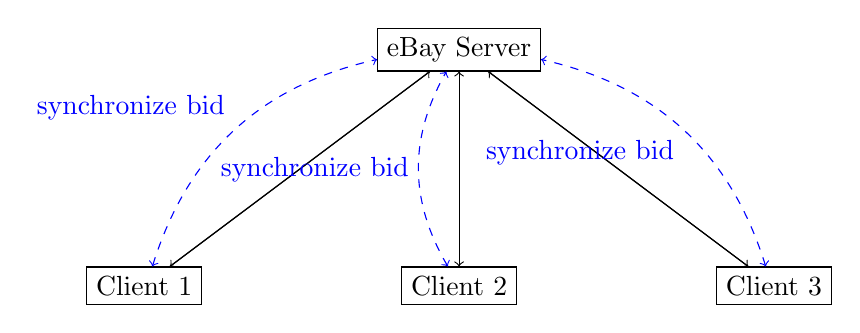
\begin{tikzpicture}[node distance=3cm, auto]
    % Nodes
    \node (ebay) [rectangle, draw] {eBay Server};
    \node (client1) [rectangle, draw, below of=ebay, xshift=-4cm] {Client 1};
    \node (client2) [rectangle, draw, below of=ebay] {Client 2};
    \node (client3) [rectangle, draw, below of=ebay, xshift=4cm] {Client 3};

    % Arrows
    \draw[->] (client1) -- (ebay);
    \draw[->] (client2) -- (ebay);
    \draw[->] (client3) -- (ebay);
  \draw[->] (ebay) -- (client1);
    \draw[->] (ebay) -- (client2);
    \draw[->] (ebay) -- (client3);
    \draw[blue, dashed, <->, bend left] (client1) to node {synchronize bid} (ebay);
    \draw[blue, dashed, <->, bend left] (client2) to node {synchronize bid} (ebay);
    \draw[blue, dashed, <->, bend right] (client3) to node {synchronize bid} (ebay);
\end{tikzpicture}
\end{minipage}	
\end{example}

\subsection{Message Passing}
\subsubsection{What is a Message?}
\textbf{Definition:} A message is any form of information or data that is transmitted between hosts in a distributed system. At a high level, this can be considered as any sequence of bits (ones and zeros).

\subsubsection{Uses}
Message passing is crucial for designing and implementing distributed systems. Common uses include:

\begin{enumerate}[itemsep=1pt, topsep=1pt]
    \item \textbf{Synchronization between Hosts:} Ensuring that multiple hosts have a consistent view of data or state, at least momentarily.
    \item \textbf{Data Dissemination:} Broadcasting data to multiple hosts, making sure all hosts receive the relevant information. This is very similar to synchronization of data.
    \item \textbf{Notifications of Events:} Informing hosts about specific events, such as a printer coming online or a mobile device receiving a notification.
    \item \textbf{Information Retrieval:} Requesting data from a server, which is the foundation of most HTTP traffic.
    \item \textbf{Sneakernet}: Even physically delivering data with, for example, a USB key, is considered message passing.
\end{enumerate}

\subsubsection{How to Send Messages?}
\begin{enumerate}
    \item \textbf{Push:}
    \begin{enumerate}[itemsep=0.5pt,topsep=0pt]
        \item \textit{Description:} Announcements where data is sent to peers without expecting a direct response. It's a one-way message, like a notification that might say, \texttt{"I am here."}
        \item \textit{Example:} A laptop sending a one-way message to a server, which might then do things but does not need to reply.
        \item \textit{Use Case:} Typically used in peer-to-peer problems where a response might not be necessary. An example is using \texttt{DHCP} and \texttt{multicast DNS}.
        \item \textit{Technical Considerations:} Often implemented with protocols like \textit{UDP}, where delivery is not guaranteed.
    \end{enumerate}

    \item \textbf{Pull:}
    \begin{enumerate}[itemsep=0.5pt,topsep=0pt]
        \item \textit{Description:} A request/response protocol where a client requests a resource and receives that resource.
        \item \textit{Example:} HTTP traffic, where a client requests a website and receives the text of the website.
        \item \textit{Use Case:} Common in client-server models, such as fetching a webpage. The key is that communication happens on request.
    \end{enumerate}

    \item \textbf{Push/Pull:}
    \begin{enumerate}[itemsep=0.5pt,topsep=0pt]
        \item \textit{Description:} A combination where hosts can both announce (push) and respond to requests (pull).
        \item \textit{Example:} Peer-to-peer networks where hosts act as both clients and servers.
        \item \textit{Challenges:} Implementing this in a distributed system can be complex, requiring careful consideration of synchronization and consistency.
    \end{enumerate}
\end{enumerate}

\subsubsection{Blocking and Non-Blocking}
\begin{enumerate}
    \item \textbf{Blocking:}
    \begin{itemize}[itemsep=0.5pt,topsep=0pt]
        \item The sender waits for a response before proceeding. The operation blocks other processes until it completes. For Example, Logging into a server; the client sends a password and must wait for validation before proceeding.
        \item \textit{Use Case:} Necessary when the response is critical for subsequent actions.
    \end{itemize}
    
    \item \textbf{Non-blocking:}
    \begin{itemize}[itemsep=0.5pt,topsep=0pt]	
        \item The sender does not wait for a response and continues other operations. For Example, Requesting images from a webpage after the initial HTML is loaded.
        \item \textit{Use Case:} Useful when immediate response is not critical, allowing for concurrent operations and improved efficiency.
    \end{itemize}
\end{enumerate}

\subsubsection{Rendezvous}

Rendezvous involves synchronizing state between a client and a server. The client waits for a response (e.g., during login).

\subsubsection{Call Back}

A callback is an asynchronous request. The client sends a request and continues execution while the server processes the request and eventually sends a response.  This is a non-blocking approach.

\subsubsection{Relay Buffer}

In a relay system, a request might travel from host 1 to host 2 to host 3, and the response follows the same path.  This is common in location transparency with web proxies.  Host 1 sends a message and blocks, waiting for a response from host 2. Host 2, in turn, sends a request to host 3 and blocks.

\textbf{Flooding} is a very simple algorithm. If you receive a message you forward the message to every node connected to you, except for the one that you just received the message from. It works well if the number of nodes is small, but the number of messages quickly becomes large.

\textbf{Gossiping} is just like flooding, but you only send the message to a few neighbours.

\subsection{Dijkstra's Algorithm}

Dijkstra's algorithm is a well-known algorithm for finding the shortest paths between nodes in a graph.

\begin{itemize}
    \item \textbf{Algorithm Steps:}
    \begin{enumerate}[itemsep=1pt, topsep=1pt]
        \item Find the current minimum cost node.
        \item "Push" the cost to get to this point plus the cost to all its peers.
    \end{enumerate}
    \item \textbf{Distributed Implementation:} In a distributed system, implementing Dijkstra's algorithm is complex because there is no shared memory.
\end{itemize}
We have a min-heap or a min-queue, but it is not trivial to understand where it is or how to synchronize the data.
\endclass{Week 2}